\documentclass[a4paper, 12pt]{article}

\usepackage[portuguese]{babel}
\usepackage[utf8]{inputenc}
\usepackage{mathtools}
\usepackage{indentfirst}
\usepackage{graphicx}
\usepackage{enumerate}
\usepackage[cache=false]{minted}
\usepackage[colorlinks=true]{hyperref}

\begin{document}

%\maketitle
  
\begin{titlepage}
\begin{center}
  \huge{Instituto Federal de Educação, Ciência e Tecnologia de Alagoas}
  
  \vspace{10pt}
  \begin{figure}[!ht]
    \centering
    
\includegraphics[height=2cm, width=7cm]{logo.jpg}
  \end{figure}
  
  \vspace{85pt}
  
  \textbf{\LARGE{Emotion Recognition}}\\
  \large{Computação Gráfica}
  \vspace{160pt}
  
\end{center}

\begin{flushleft}
  \begin{tabbing}
    Alunos\qquad\qquad\= Djalma Júnior\\
    \>Djanilson Alves\\
    Professor\> Leonardo Medeiros \\
  \end{tabbing}
\end{flushleft}

\begin{center}
  \vspace{\fill}
  Maceió, \today
\end{center}
\end{titlepage}

%%%%%%%%%%%%%%%%%%%%%%%%%%%%%%%%%%%%%%%%%%%%%%%%%%%%%%%%%%%%

\newpage
\tableofcontents
\thispagestyle{empty}

\newpage
\pagenumbering{arabic}

%%%%%%%%%%%%%%%%%%%%%%%%%%%%%%%%%%%%%%%%%%%%%%%%%%%%%%%%%%%%

\section{Objetivos}

\section{Tecnologias utilizadas}

\subsection{OpenCV + DLib + SKLearn}

O OpenCV possui algumas classes de reconhecimento de face do qual usaremos o \href{http://www.scholarpedia.org/article/Fisherfaces}{FisherFace}. \href{http://dlib.net/}{Dlib} também é uma biblioteca para reconhecimento de faces cuja técnica consiste em marcar o rosto com pontos indicando as regiões da face (como olhos, boca, nariz, etc).

Essas duas bibliotecas serão utilizadas para o reconhecimento de emoções e comparadas para verificar qual delas chegam mais próximo do resultado desejado. Usaremos o dlib em conjunto com um algoritmo de aprendizado de máquina do \href{http://scikit-learn.org/stable/}{sci-kit learn}.

\subsection{CK Dataset}

O conjunto de dados \href{http://www.pitt.edu/~emotion/ck-spread.htm}{Cohn-Kanade} será utilizado como base para o treinamento dos classificadores.

\section{Procedimento}

\subsection{Organizando os dados}

Inicialmente, foi necessário organizar o \textit{dataset}. No diretório do projeto foram criadas duas pastas chamadas \textit{emotions} e \textit{images}. Os dados contendo os arquivos \textit{.txt} (S005, S010, etc.) ficaram na pasta \textit{emotions} e as imagens em \textit{images}. Também foi criada uma pasta chamada \textit{sorted} para armazernar as imagens de emoções ordenadas por nome (\textit{neutral}, \textit{anger}, etc.). 

No arquivo \textit{readme}, os autores do \textit{dataset} mencionam que apenas um subconjunto (327 do 593) das seqüências realmente contém as emoções. Cada sequência de imagens consiste na formação de uma expressão emocional, começando com um rosto neutro e terminando com a emoção. Então, a partir de cada sequência de imagens, extraímos duas imagens: uma neutra (a primeira imagem) e uma com a expressão emocional (a última). Para ajudar a fazer essa separação, foi necessário um pequeno script:

\inputminted[
frame=lines,
framesep=2mm,
baselinestretch=1.2,
fontsize=\footnotesize,
linenos
]{python}{sort_emotions.py}

\subsection{Preparandos as imagens}

Para que os classificadores funcionem melhor, as imagens precisam estar no mesmo tamanho e ter apenas um rosto nelas. Os passos para isso são: a) encontrar o rosto em cada imagem, b) converter em escala de cinza, c) recortar, redimensionar e salvá-las em outro diretório. 

Para automatizar a busca da face, foi utilizado um filtro HAAR do OpenCV. O OpenCV fornece 4 classificadores pré-treinados, por isso, para ter certeza de que a busca da face será eficaz, todos os filtros foram utilizados em sequência e, assim que uma face for encontrada, descartamos os demais resultados.

Essa extração das faces se dá com o seguinte \textit{script}:

\inputminted[
frame=lines,
framesep=2mm,
baselinestretch=1.2,
fontsize=\footnotesize,
linenos
]{python}{extract_faces.py}

O último passo foi filtrar o nosso \textit{dataset}. Como a maioria dos participantes tem várias amostras de expressões, temos algumas repetidas imagens da mesma pessoa. Neste caso, o trabalho de remoção foi manual.

\section{Extraindo características das faces}

Para treinar nosso datase usando dlib, foi necessário extrair algumas características da imagem para que o classificador trabalhe corretamente. A forma que foi feita essa extração da informação foi obtendo as coordenadas do ponto central do rosto e, em seguida, obter a posição de todos os pontos relativos a este ponto central. Isso se faz necessário para evitar que o classificador trabalhe com o posicionamento absoluto dos pontos, visto que a pessoa pode apresentar a mesma expressão, porém os pontos estão em posições diferentes da tela. As faces também podem estar inclinadas, o que pode confundir o classificador. Foi feita um correção simples para amenizar esse problema.

\section{Rodando o experimento}

O código principal do programa é o seguinte:

\inputminted[
frame=lines,
framesep=2mm,
baselinestretch=1.2,
fontsize=\footnotesize,
linenos
]{python}{main.py}

\subsection{Acuracidade}

Para obter a acuracidade dos algorítmos, foi obtido aleatoriamente 80\% das imagens e os 20\% restantes foram classificadas para efeito de comparação. Esse processo foi repetido 10 vezes. Os scripts \texttt{accur\_fishface.py} e \texttt{accur\_landmarks.py} são utilizados para fazer esses cálculos.

A precisão do reconhecimento usando a técnica de fishface obteve uma média de 69.9\% (figura \ref{fig:fishface}). Utilizando landmarks, 71,5\% (figura \ref{fig:landmarks}).

\section{Análise dos resultados e conclusão}

A primeira coisa a se notar é que temos poucos exemplos de emoções. Isso faz com que os classificadores não tenham uma precisão muito boa e informe incorretamente a emoção obtida pela câmera. Usar um conjunto de dados maior provavelmente aumentará bastante a detecção. Além do mais, o \textit{dataset} não condiz exatamente com uma emoção que as pessoas fazem no dia a dia. Algumas dessas imagens chegam até a ser cômicas.

É claro que o reconhecimento de emoção é uma tarefa complexa, mais ainda quando só usa imagens. Mesmo para nós humanos, isso é difícil porque o reconhecimento correto de uma emoção facial muitas vezes depende do contexto dentro do qual a emoção se origina e se expressa.

O repositório desse projeto pode ser encontrado em \url{https://github.com/djalmajr/emotion-recognition}

\newpage
\section{Figuras}

\begin{figure}[!ht]
  \centering
  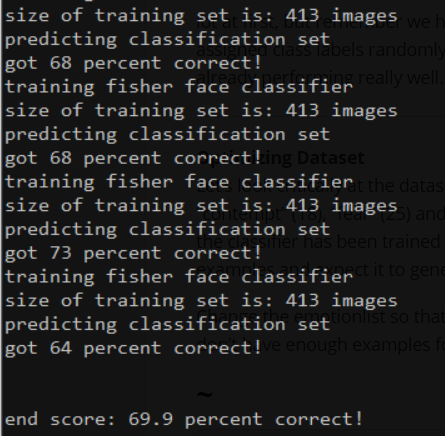
\includegraphics[height=6cm, width=6cm]{fishface.png}
  \caption{Precisão utilizando fishface}
  \label{fig:fishface}
\end{figure}

\begin{figure}[!ht]
  \centering
  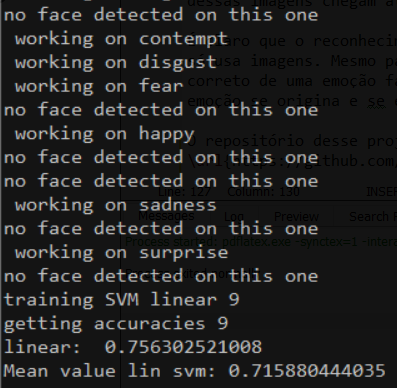
\includegraphics[height=6cm, width=6cm]{landmarks.png}
  \caption{Precisão utilizando landmarks}
  \label{fig:landmarks}
\end{figure}

\newpage
\section{Referências}

van Gent, P. (2016). Emotion Recognition With Python, OpenCV and a Face Dataset. Retrieved from: http://www.paulvangent.com/2016/04/01/emotion-recognition-with-python-opencv-and-a-face-dataset/ \\

Adrian Rosebrock, (2017). Facial landmarks with dlib, OpenCV, and Python. Retrieved from: https://www.pyimagesearch.com/2017/04/03/facial-landmarks-dlib-opencv-python/

\end{document}